\documentclass[11pt,a4paper]{article}
\usepackage[margin=18mm]{geometry}
\usepackage[T1]{fontenc}
\usepackage{newtxtext,newtxmath}
\usepackage{microtype,graphicx,booktabs,caption,xcolor,hyperref}
\usepackage{enumitem}
\hypersetup{colorlinks=true,urlcolor=teal,citecolor=teal,linkcolor=black}
\graphicspath{{figures/}}
\setlength{\parindent}{0pt}
\setlength{\parskip}{5pt}
\captionsetup{font=small,labelfont=bf,skip=4pt,hypcap=false}
\setlist{nosep,leftmargin=*}
\newcommand{\papersection}[1]{\vspace{5pt}{\large\bfseries #1}\par\vspace{1pt}}
\newcommand{\AbstractResults}{ApiaViz completed three of four routes, whereas
Sobel filtering with colour completed all four. ApiaViz had lower average
tracking error (11.5 versus 18.5\,cm, including failures). These results show
that deterministic spiking representations can support navigation, but do not
establish an overall advantage for ApiaViz over simple filtering.}

\newcommand{\ResultsParagraph}{ApiaViz reached the nest on three routes;
Sobel plus colour reached it on all four. Grayscale also completed three routes,
while raw colour, simple opponency and Ardin-style input each completed two.
ApiaViz's mean route
deviation was 11.5\,cm, compared with 18.5\,cm for Sobel and 33.1\,cm for grayscale.
Ardin-style input had a mean deviation of 66.4\,cm.
ApiaViz and Sobel produced similar activity levels: 4.95\% of KCs for
ApiaViz and 4.99\% for Sobel. Their different outcomes therefore occurred at
similar average sparsity.}

\newcommand{\DiscussionOpening}{The comparison separates two useful outcomes:
staying close to the taught route and eventually reaching the nest. ApiaViz
tracked three routes closely but failed on Ant~8. Sobel completed that route
and the other three, although its Ant~11 trial took 183 steps and had a mean
deviation of 53.6\,cm. ApiaViz may help tracking precision, but this experiment
does not show that it is a more reliable navigation input than Sobel filtering.}

\newcommand{\ConclusionParagraph}{A deterministic spiking navigation system
is feasible in this setting. ApiaViz reduced tracking error, while Sobel
produced the most consistent completion. Recovery after drift is therefore
the immediate priority for ApiaViz, followed by tests across more environments
and neural wiring seeds with the same matched controls.}

\begin{document}
\thispagestyle{plain}
{\LARGE\bfseries ApiaViz: colour and contrast preprocessing\par
for spiking visual navigation\par}
\vspace{4pt}
{\small Preliminary simulation study\hfill 29 September 2026}
\vspace{5pt}\hrule\vspace{5pt}

{\small\textbf{Abstract.}
Insect-inspired navigation models often reduce an image to a small set of pixel
intensities before forming a sparse neural representation. ApiaViz adds fixed
colour and local-contrast processing. We compared six image-processing methods
on the same four simulated routes, keeping route learning, spiking neurons,
memory and steering unchanged. The visual filters were not trained.
\AbstractResults\par}

\papersection{1\quad Motivation}
A mushroom body is an insect brain structure involved in learning associations.
Its Kenyon cells represent inputs through the activity of relatively few neurons.
For navigation, a useful representation must distinguish nearby views while
still allowing an animal to recognise a familiar route after moving.
Ardin et al.~[1] showed how sparse visual activity can support route memory.
More recently, Gattaux et al.~[2] combined Sobel edge filtering with directional
memories and velocity control on a robot. These studies motivate a practical
question: does ApiaViz provide a better visual input to the memory system than
simpler processing?

\papersection{2\quad Methods}
We used four approximately 8\,m routes in a reconstructed grassland with synthetic
coloured landmarks (Ants 5, 8, 11 and 14, Route 2). Each condition learned from
exactly the same images: nine lateral viewpoints spanning $\pm20$\,cm at each
10\,cm route interval, facing along the route. Learning recorded each sparse
pattern once. No visual weights or neural connections were fitted.

\begin{center}
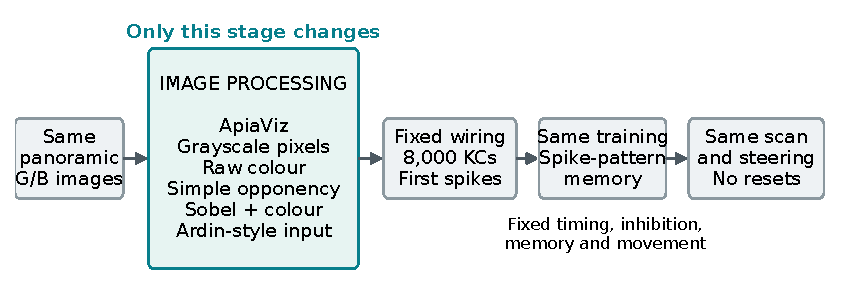
\includegraphics[width=\linewidth]{methodology.pdf}
\captionof{figure}{\textbf{Controlled input substitution.} Green and blue (G/B)
image channels enter one of six preprocessing methods. The route-learning
images, neural connections, spike parameters, memory rule and movement policy
are identical across conditions. KCs: Kenyon cells.}
\end{center}

Every method supplied five image maps, pooled to $8\!\times\!64$ and
standardised within each of two input streams. ApiaViz used
hexagonal spatial averaging, local brightness adaptation, centre--surround
contrast and green--blue opponency. Controls used grayscale pixels, raw colour,
simple colour differences, Sobel gradients plus colour differences, or
Ardin-style inverted, locally equalised $10\!\times\!36$ intensity images.
Single-channel inputs were copied across the maps so neither KC population
was left unused. The Ardin condition applies the published image operations
within our shared test pipeline.

\newpage
\papersection{2\quad Methods (continued)}
All conditions used the same fixed random connections to 8,000 leaky
integrate-and-fire KCs: model neurons that accumulate input until firing.
Each KC sampled ten inputs and could emit one spike per
50\,ms presentation. Spike times had 1\,ms resolution, with a 1\,ms inhibitory
delay. Current gain and the inhibition trigger were fixed at the previously
selected ApiaViz values for every method. We measured the resulting activity
instead of forcing all outputs to have identical sparsity.

The common memory stored which KCs fired in each teaching view. Recall counted
active cells shared with each stored pattern, normalised by the pattern sizes.
Each route stored 693--747 patterns. The agent scanned 13 headings across $\pm60^\circ$ and moved 10\,cm
towards the most familiar view. No position or heading resets were allowed.
An evaluator counted arrival within 20\,cm of the nest as success, with a
200-step limit. Thus navigation remained visually guided but received no
external route corrections (the project's ``open-loop'' condition).

\papersection{3\quad Results}
\ResultsParagraph

\begin{center}
\IfFileExists{figures/comparison.pdf}{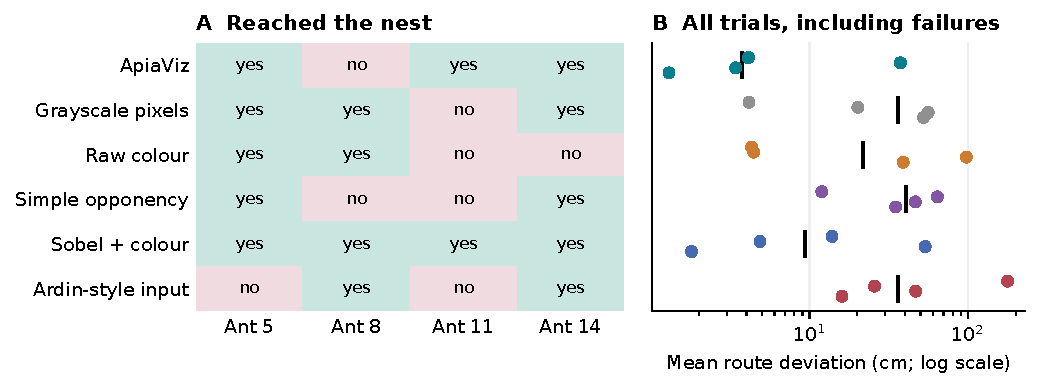
\includegraphics[width=\linewidth]{comparison.pdf}}{\fbox{\parbox[c][6cm][c]{.95\linewidth}{\centering Analysis in progress}}}
\captionof{figure}{\textbf{Open-loop comparison on the same routes.} (A) Nest
arrival within 200 steps. (B) Each point is one route's mean distance from the
taught centreline; black marks indicate medians. Failed trials are included.
Distances are computed to the nearest route sample, spaced 10\,cm apart.}
\end{center}

\begin{center}
\small\begin{tabular}{@{}lrrr@{}}\toprule
Image preprocessing & Completed & Mean deviation & Active KCs \\
 & (of 4) & (cm) & (\%) \\\midrule
ApiaViz & 3/4 & 11.5 & 4.95 \\
Grayscale pixels & 3/4 & 33.1 & 5.51 \\
Raw colour & 2/4 & 36.3 & 5.52 \\
Simple opponency & 2/4 & 39.3 & 5.36 \\
Sobel + colour & 4/4 & 18.5 & 4.99 \\
Ardin-style input & 2/4 & 66.4 & 5.55 \\
\bottomrule\end{tabular}

\captionof{table}{All four trials contribute to each mean. Activity is the
fraction of KCs that fired during route learning. The same inhibition settings
were used throughout; differences in actual activity arise from preprocessing.}
\end{center}

The ApiaViz reruns reproduced their previously recorded trajectories exactly.
Recorded training-image hashes, steering scores and movement traces allow the comparison
to be checked independently.

\newpage
\papersection{4\quad Discussion}
\DiscussionOpening

\begin{center}
\IfFileExists{figures/trajectories.pdf}{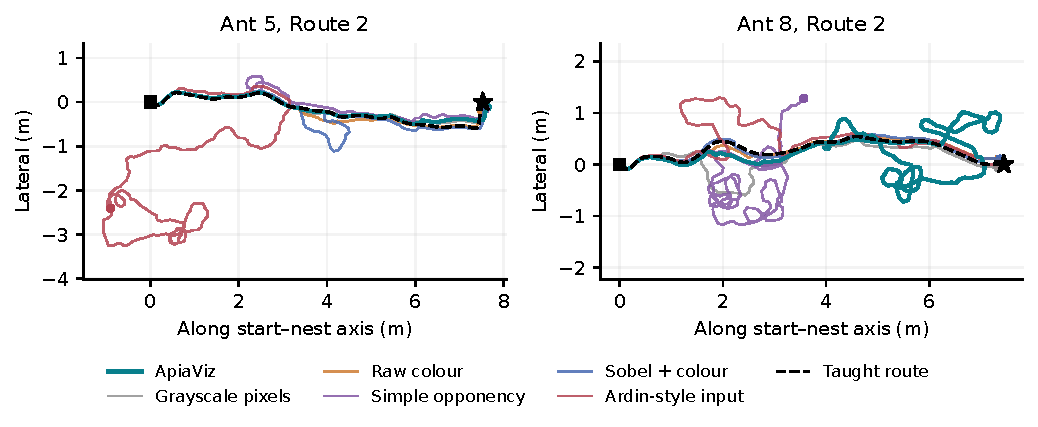
\includegraphics[width=\linewidth]{trajectories.pdf}}{\fbox{\parbox[c][6cm][c]{.95\linewidth}{\centering Analysis in progress}}}
\captionof{figure}{\textbf{Examples of route following and failure.} Ants 5 and 8
were chosen for illustration before observing baseline outcomes. Dashed lines
show the taught routes; squares mark starts and stars mark nests. Coloured dots
mark final positions. Coordinates are rotated to place the nest to the right
of the start. Figure~2 and Table~1 include all four tested routes.}
\end{center}

The matched Ardin-style condition answers a narrower question than a comparison
with the original paper: what happens when its image preprocessing feeds our
shared encoder and memory? Ardin et al.~[1] used a different spiking circuit and
corrected route departures beyond 20\,cm. Its published results should therefore
not be interpreted as unassisted completion scores in this experiment. Likewise,
our colour-preserving Sobel condition does not reproduce the Antcar controller
of Gattaux et al.~[2].

This pilot covers four routes in one simulated world, with one connectivity
seed and aligned starting poses. Recovery from displacement and changes in
illumination require further tests. Neural settings were selected earlier for
ApiaViz and then held fixed across all input substitutions. The comparison
therefore describes performance at one shared setting. Template storage also
uses more memory than a compact mushroom-body output circuit. The visual
filters, signed input projection and memory readout use graded values; only the
KCs emit spikes.

\ConclusionParagraph

\vspace{5pt}
{\small\textbf{References}\par
[1] P. Ardin, F. Peng, M. Mangan, K. Lagogiannis and B. Webb (2016).
Using an insect mushroom body circuit to encode route memory in complex natural
environments. \emph{PLOS Computational Biology} 12, e1004683.
\href{https://doi.org/10.1371/journal.pcbi.1004683}{doi:10.1371/journal.pcbi.1004683}.\par
[2] G. G. Gattaux, A. Wystrach, J. R. Serres and F. Ruffier (2025).
Route-centric ant-inspired memories enable panoramic route-following in a
car-like robot. \emph{Nature Communications} 16, 8328.
\href{https://doi.org/10.1038/s41467-025-62327-3}{doi:10.1038/s41467-025-62327-3}.\par}
\end{document}
